\documentclass[a4paper,12pt]{ctexart}     %页面大小和字体大小

\usepackage{ctex}
\usepackage{mathptmx}
\usepackage{amsmath}

\usepackage{url}  % 添加网页

\usepackage{listings}  %添加代码
% 设置代码格式
\usepackage{xcolor}
\lstset{
	language=R,
	backgroundcolor=\color{white}, 
	numbers=left, 
	numberstyle= \tiny, 
	keywordstyle= \color{ blue!70},
	commentstyle= \color{red!50!green!50!blue!50}, 
%	frame=shadowbox, % 阴影效果
	rulesepcolor= \color{ red!20!green!20!blue!20} ,
	escapeinside=``, % 英文分号中可写入中文
	xleftmargin=2em,xrightmargin=2em, aboveskip=1em,
	framexleftmargin=2em
} 

\usepackage{graphicx} %插入图片的宏包
\usepackage{float} %设置图片浮动位置的宏包
\usepackage{subfigure} %插入多图时用子图显示的宏包


\usepackage{booktabs}  % 三线表


\usepackage{geometry}
\geometry{left=3.17cm, right=3.17cm, top=2.54cm, bottom=2.54cm}   %页边距
\linespread{1}      %设置行距


% 摘要设置  -->设置为4号字
\renewcommand{\abstractname}{\textbf{\zihao{4}摘\quad 要}}

% 设置标题
\ctexset{
	section={
		format=\bfseries\zihao{4}\heiti\centering
	}
}

% 设置目录
\setcounter{tocdepth}{2} %设定目录深度为2,即只显示到二级标题为止

% 设置页码
\pagestyle{plain}

\begin{document}\songti\zihao{5}
	{\zihao{3}\heiti
	\title{基于R语言的爬虫和基本文本分析}
	\date{}
	\maketitle
	}
	

%	\begin{abstract}
%		随着大数据时代的到来,互联网上产生了越来越多的数据具有很大的参考价值,这些数据中往往蕴含着充分的政治、经济、社会人文等各种充满价值的信息,如果充分利用互联网信息来解读社会发展脉络,提炼其背后所蕴含的信息意义重大。本文基于R语言通过网络爬虫技术,获取了上海对外经贸大学一微信公众号平台的文本评论,然后通过对文本进行分词和去停用词处理,得到具有价值的文本信息,后对文本进行词频统计,可以获得该用户群体的热点词汇,然后根据词频对词汇绘制词云,获得可视化效果,后一步对文本进行主题分析、情感分析等奠定了基础。
%		
%		\vspace*{1\baselineskip}   %空白间距
%		
%		\noindent{\textbf{关键词:}爬虫\quad 词频统计 \quad 绘制词云 }
%	\end{abstract}

	\tableofcontents  %目录部分
	\newpage   %新页
	\section{基本任务描述}

随着大数据时代的到来,互联网上产生了越来越多的数据具有很大的参考价值,这些数据中往往蕴含着充分的政治、经济、社会人文等各种充满价值的信息,如果充分利用互联网信息来解读社会发展脉络,提炼其背后所蕴含的信息意义重大。本文的任务是通过爬虫技术获取网页数据,然后对获取的数据进行数据清洗,数据处理相关工作,然后对该数据进行基本的统计分析,以获得数据中所获得的有价值的信息。此次获取的是上海对外经贸大学活跃度较高、在同学之间名气较为旺盛的微信公众号——大猫助手pro的网页评论,该评论由于是非官方平台且采用匿名制,较能反映出大学生内的真实想法,具有较强的舆情价值。

	

	\section{设计思路}

	本文通过R语言中的爬虫程序来获取和解析网页内容,本文在线抓取了自3月份至6月份一共70天的数据,获得1453条学生评论,然后通过jieba对每条内容进行分词,由于平日用语中的类似助词等的词汇,但是这些词汇我们并不感兴趣,所以通过载入停用词表( 可以在附录中网址获得 ),去除这些停用词,然后就可以对文本进行基本的统计,获取出现评率最高的词汇。频率最高的词汇并不一定是最重要的词汇,此时引入逆文档频率的相关概念,然后得到更为重要的关键词,通过绘制词云获得可视化效果,以此来推断该群体的状况与舆论态势,可以进行很多工作。设计的流程图如图1所示。
	
		\begin{figure}[H] %H为当前位置,!htb为忽略美学标准,htbp为浮动图形
			\centering %图片居中
			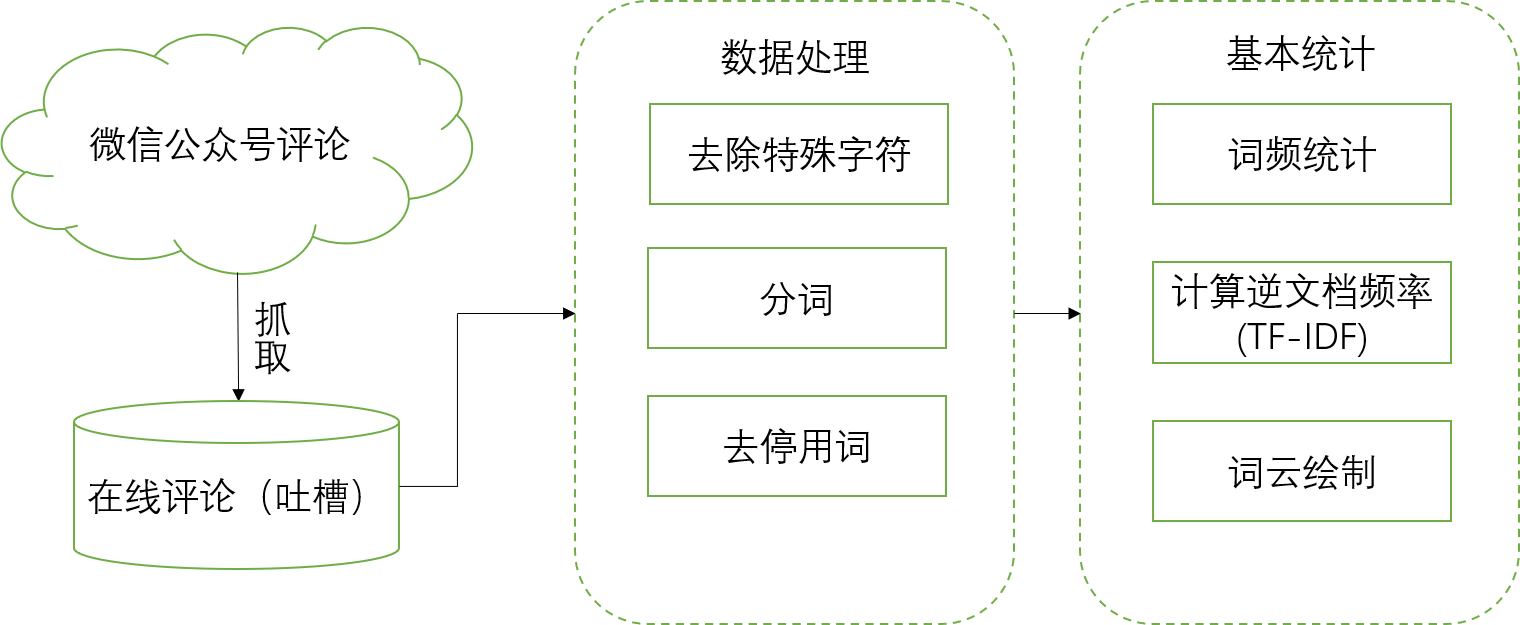
\includegraphics[width=0.7\textwidth]{流程图.png} %插入图片,[]中设置图片大小,{}中是图片文件名
			\caption{设计流程图} %最终文档中希望显示的图片标题
			\label{Fig.main 1} %用于文内引用的标签
		\end{figure}




	\section{文本获取}
	
	爬虫的基本原理是模拟浏览器发送请求,然后下载网页代码(本文所使用的网页的URL可的网址下载获取),R语言有丰富的包可以实现获取网页代码,本文采取的是rvest包来获取,然后利用RCurl包中的html\_nodes 函数来提取网页中有用的内容,由于评论较为简短,
	所以在附录中以把每一条评论存放在一个数据框中
	
	\section{文本处理}
	
	\subsection{去除特殊字符与分词}
	
	到目前为止我们所获取的还是整句的评论,想要进一步分析评论所蕴含的信息,我们要对评论进行分词处理。注意到评论中含有的表情符号解析后是由特殊字符和数字构成的,这对分词结果会造成影响,所以我们应该首先除去这些特殊字符,这里本文采用的是通过正则提取的方式去除这些特殊字符。而后对每一条评论进行分词。分词所采用的工具是R语言中的jiebaR库来实现,jiebaR库一共提供7种分词引擎,在本文中采取的是混合模型。它混合使用了最大概率法和隐式马尔科夫模型,是目前分词较为准确的一种。对所有评论分词之后一共获取29383个词汇,部分结果显示如图2所示。
	
		\begin{figure}[H] %H为当前位置,!htb为忽略美学标准,htbp为浮动图形
			\centering %图片居中
			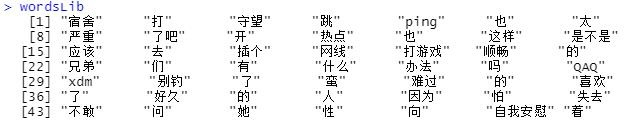
\includegraphics[width=0.7\textwidth]{分词结果.jpg} %插入图片,[]中设置图片大小,{}中是图片文件名
			\caption{部分分词结果} %最终文档中希望显示的图片标题
			\label{Fig.main 2} %用于文内引用的标签
		\end{figure}
	
	\subsection{去停用词与非中文词}
	
		从分词结果中我们可以看到类似“了”、“的”之类的助词对我们进行文本分析是没有帮助的,所以我们必须去除这些对于文章内容理解无关紧要的词汇,本文通过载入停用词表的方式对分词之后的文本进行匹配(本文所使用停用词表可以在附录网页中下载获取)如果文本中出现在停用词表中,则去除这些词汇,通过去停用词之后,剩下16779个关键词汇。部分结果显示如图3所示。
		
		\begin{figure}[H] %H为当前位置,!htb为忽略美学标准,htbp为浮动图形
			\centering %图片居中
			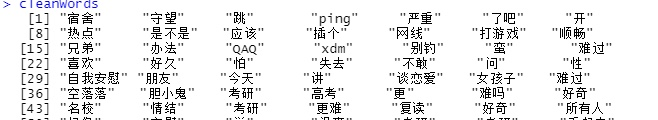
\includegraphics[width=0.7\textwidth]{去停用词后结果.png} %插入图片,[]中设置图片大小,{}中是图片文件名
			\caption{去停用词后结果} %最终文档中希望显示的图片标题
			\label{Fig.main 3} %用于文内引用的标签
		\end{figure}
		从分词结果可以看出,分词对结果有较大影响,对更准确把握文本内容具有重大意义。		
	\subsection{词性标注}
	
	到目前为止已经完成了关键词的提取,我们还可以对关键词的进行词性标注,加深对文本内容的把握。对这一目标的实现使用了R语言的tmcn库中的vector\_tag函数,可以实现对每个词的词性标注,截取频率前十的词性绘制条形图,结果如图4(a)所示
	
	
		
	\begin{figure}[htbp]
		\centering
		\subfigure[词性统计]{
			\begin{minipage}[t]{0.5\linewidth}
				\centering
				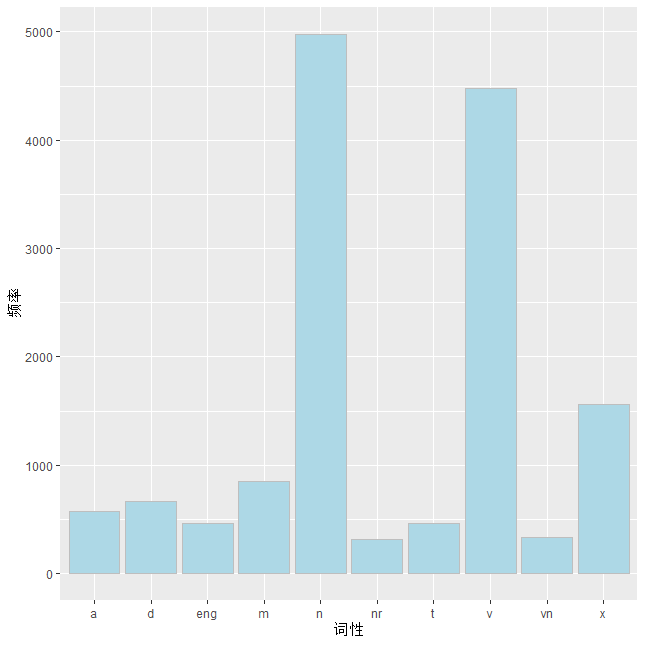
\includegraphics[width=0.7\textwidth]{词性统计.png}
				%\caption{fig1}
			\end{minipage}%
		}%
		\subfigure[词频统计]{
			\begin{minipage}[t]{0.5\linewidth}
				\centering
				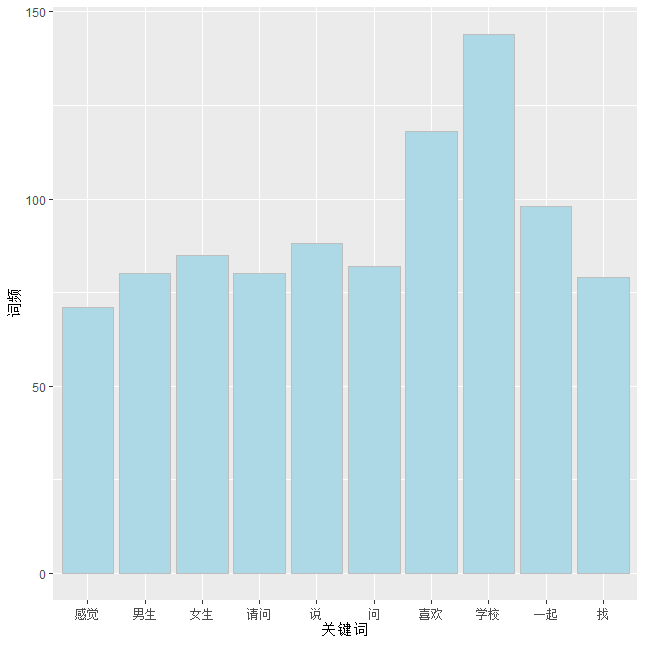
\includegraphics[width=0.7\textwidth]{词频统计.png}
				%\caption{fig2}
			\end{minipage}%
		}%
		\centering
		\caption{基本统计}
	\end{figure}
	
	\section{基本统计}

	\subsection{词频统计}
	
	完成了对文本的预处理工作之后,我们需要进行处理后的内容进行基本的统计,首先是对词频的统计,经过去停用词之后选取频率前十的词语绘制条形图,结果如图4(b)所示。为了获得更好的可视化效果,选取频率前50的词语,绘制词云图,结果如图5所示。

%	\begin{table}[htbp]   
%		\caption{\label{tab:test}示例表格} 
%		\begin{center}
%			\begin{tabular}{llll}   
%				\toprule    
%				评论相关属性 & 最小值 & 最大值&  平均值 \\    
%				\midrule   
%				。。 & 。。 & 。。&  。。 \\   
%				。。 & 。。 & 。。&  。。 \\   
%				。。 & 。。 & 。。&  。。 \\    
%				\bottomrule   
%				
%			\end{tabular} 
%		\end{center}
%		\label{tbl:table-example} 
%	\end{table}
%	
	
	\begin{figure}[H] %H为当前位置,!htb为忽略美学标准,htbp为浮动图形
		\centering %图片居中
		
\includegraphics[width=0.7\textwidth]{词云图.png} %插入图片,[]中设置图片大小,{}中是图片文件名
		\caption{词云图} %最终文档中希望显示的图片标题
	\end{figure}
	
	\subsection{计算关键词重要性TF-IDF}
	前面所作的工作都是为了提取每个词语的频率,但是词语出现的频率越高,不一定代表该词越重要,相反的是在一些特殊的文章中,某些词语虽然频率在这篇文档中不是最高的,但是在其他文档中比较少见,说明这种词汇反映了该文章的特性,为了描述这种现象,引入逆文档频率的概念。
	
	在词频(Term Frequency)基础之上,设置一个重要性调整系数,对较少见的词给予较大的权重,即逆文档频率(Inverse Document Frequency)简称IDF,而后提出关键词重要性(TF-IDF),是由词频和逆文档频率的乘积定义,用这个指标提取文本中的关键词。
	为了便于解释,特对符号进行说明,如表1所示。
		\begin{table}[htbp]   
		
			\begin{center}
				\begin{tabular}{ll}   
					\toprule    
					属性 & 符号  \\    
					\midrule 
					词汇频率 & TF \\  
					逆文档频率 & IDF  \\   
					语料库的文档总数 & sumCorpus  \\   
					包含该词的文档数 & incCorpus  \\
					关键词重要性 & IF-IDF\\  
					\bottomrule   
					
				\end{tabular} 
				\caption{\label{tab:test}符号说明} 
			\end{center}
		\end{table}
	
逆文档频率的计算方法为
$$
IDF = log(\frac{sumCorpus}{invCorpus+1})
$$
\par
关键词重要性的计算方法为
$$
TF-IDF = TF \times IDF
$$
\par
本文所采用的语料库是jiebaR库中所带有的语料库,经过计算之后,提取重要性前二十的词汇绘制条形图,如图6所示。
	
\par	
		\begin{figure}[H] %H为当前位置,!htb为忽略美学标准,htbp为浮动图形
			\centering %图片居中
			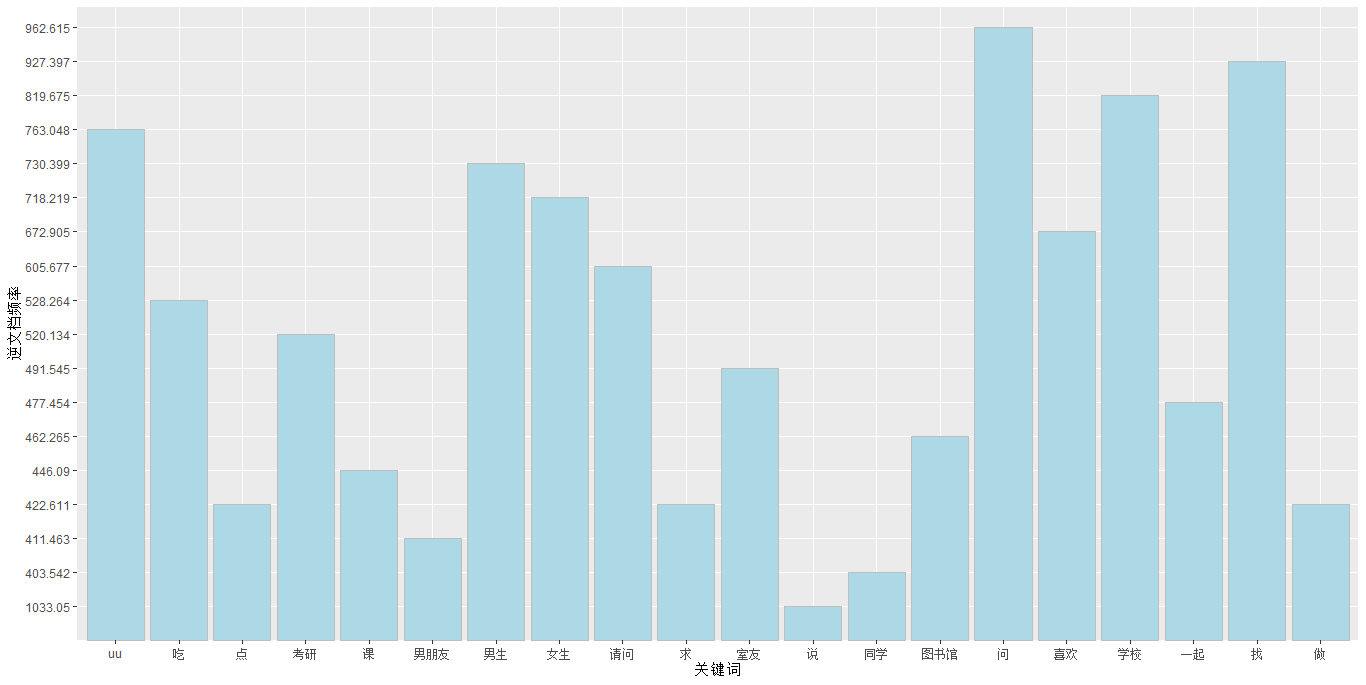
\includegraphics[width=0.7\textwidth]{逆文档频率.png} %插入图片,[]中设置图片大小,{}中是图片文件名
			\caption{逆文档频率} %最终文档中希望显示的图片标题
		\end{figure}

	


	\section{结果分析}
	由于所抓取网页的特殊性(该公众号以匿名表白而在同学之间闻名),所获取的数据本身带有一定的情感倾向,通过对文本进行基本的统计之后,发现文本内容多以情感类词汇为主,比如“喜欢”、“男朋友”、“女生”等,说明所获得的结果能够和实际情况充分印证。
	
	\section{自我评价}
	
	本文完成了最基本的网页数据的处理分析工作,但是获取数据之后对数据利用率太低,只是进行了最基本的统计,没有进一步挖掘数据背后所蕴含的信息,下一步可以对数据进行主题分析,情感分析等实现对所获取数据的高效率利用。
	
	
	\begin{thebibliography}{99}    %参考文献开始
		\par
	[1]轻松学统计,基于R语言的TF-IDF算法(文本挖掘),\url{http://blog.csdn.net/kunga0814/archive/2009/04/22/4099829.aspx} ,6(8),2021 
	\\


	[2]R语言中文社区,R语言自然语言处理:关键词提取(TF-IDF),\url{https://blog.csdn.net/kMD8d5R/article/details/88564616} ,(6)8,2021
	\\
	
	
	[3]R3eE9y2OeFcU40,R语言自然语言处理:词性标注与命名实体识别,\url{https://blog.csdn.net/R3eE9y2OeFcU40/article/details/88265401},6(8),2021
	\\
	
	
	[4]余醉 | dtminer,R语言数据可视化词云绘制,\url{https://blog.csdn.net/sinat_30361015/article/details/85876695},6(8),2021
	\end{thebibliography}

\addcontentsline{toc}{section}{参考文献}



	
	\begin{appendix}
		
		\section{附录}
		\subsection{代码}
\begin{lstlisting}
	
library(tmcn)
library("HMM")
library(rvest)  
library(RCurlibrary(openxlsx)  # read excel file
library(jiebaRD)
library("jiebaR") 
library(NLP)
library(tm)
library(RColorBrewer)
library(wordcloud2) # word cloud
library("topicmodels")
library("Rwordseg")
library("ggplot2")
library(tidyverse)  # offer enframe to transform the type of data
library(magrittr)

setwd("d:/Rdata/Crawl")

# Loading data
urlData<-read.xlsx('url.xlsx')

urlData <- as.matrix(urlData)

urlData <- urlData[1:70]

htmlData1 <- matrix()

for (turl in urlData){
	
	if(url.exists(url=turl)){
		
		hdata<-read_html(turl) 
		
		htmlData<-hdata%>%html_nodes('div.rich_media_content section 
		section section section section section 
		section section')%>%html_text()
		
		htmlData <- as.matrix(htmlData)
		
		htmlData1 = rbind(htmlData,htmlData1)
	}
}

na.omit(htmlData1)

wk = worker()

wordsLib <- c()

textLib <- data.frame()

for(i in htmlData1){
	
	tmp <- wk[i][grep("[^0-9]",wk[i],fixed=FALSE)] 
	
	textLib <- rbind(textLib)
	
	wordsLib <- c(wordsLib,tmp)
}

na.omit(wordsLib)


stopwords <- unlist(read.table("StopWords.txt",encoding = "utf-8",
fileEncoding = "utf-8"))

removeStopWords <- function(x,stopwords) {
	
	temp <- character(0)
	
	index <- 1
	
	xLen <- length(x)
	
	while (index <= xLen) {
		
		if (length(stopwords[stopwords==x[index]]) <1)
		
		temp<- c(temp,x[index])
		
		index <- index +1
		
	}
	
	return(temp)
	
}

cleanWords <-lapply(wordsLib,removeStopWords,stopwords)

cleanWords <- as.character(cleanWords)

temp <- cleanWords

temp <- which(temp == "character(0)")  

cleanWords <-cleanWords[-temp]

freSta <- freq(cleanWords)  

tag_worker = worker(type = "tag")    

wordType <- vector_tag(cleanWords,tag_worker)  

typeFre <- freq(wordType)



f <- typeFre[order(typeFre[2], decreasing = TRUE),]

ggplot(f[1:10,], aes(x=char,y= freq))+xlab(" Key Words")
+ylab("Frequency of Words") + geom_bar(
stat="identity",fill="lightblue", colour="grey")

f2 <- f[1:50,]
wordcloud2(data=f2,size = 1,minSize = 0.5,gridSize = 0,
backgroundColor = "white",color = "random-dark",minRotation = -pi/4,
maxRotation=pi/4,rotateRatio=0.4, shape='circle',ellipticity=0.65,
widgetsize=NULL)

f3 <- f[1:15,]
ggplot(f3, aes(x=char,y= freq)) + geom_bar(stat="identity",
fill="lightblue", colour="grey")


enframe(wordType) -> tag_table  

speechPart <- freq(tag_table$name)

speechPart <- speechPart [order(speechPart $freq,decreasing = TRUE),]  

ggplot(speechPart[1:10,], aes(x=char,y= freq))+xlab("Word type")+ylab(
"Frequcncy") + geom_bar(stat="identity",fill="lightblue", colour="grey")


keys = worker("keywords",topn = 20)

x <- vector_keywords(wordType,keys)  

y <- enframe(x)

ggplot(y, aes(x=value,y= name))+xlab("Key Word")+ylab(
"the value of TF-IDF") + geom_bar(stat="identity",
fill="lightblue", colour="grey")



\end{lstlisting}	
	\subsection{数据}	
	本文所需数据可从以下网址获取
	\par
	\url{https://github.com/Guanghui-hua/Rcode}
	\end{appendix}
\end{document}